% ----------------------------------------------------------
% Background
% ----------------------------------------------------------
\chapter{Background}

This background chapter starts with an overview about formal verification in contrast to conventional verification techniques based on simulation in Sec.~\ref{section:formal-verification} \TLSAY{strange sentence ... maybe something like First ... then we explain ... which is in contrast to ... ?}. An introduction to \textit{Interval Property Checking}~(IPC) and the notion of completeness in formal verification is also given. An overview of the work proposed in \cite{paper-pdd} about \textit{Property Driven Design}~(PDD) is shown in Sec.~\ref{section:PDD}.

\TLSAY{This reads more like a list of things you talk about. Try to put them into perspective, what are they used for in the scope of the thesis?} 

\section{Formal Verification}
\label{section:formal-verification}

The main goal of formal verification on digital designs is to overcome the coverage issue faced \TLREP{by classical (not-formal) verification by simulation}{with simulation based verification}. For this last one \TLSAY{What is the last one?}, functional validation of the system is achieved by applying stimuli to the input of the \textit{Design Under Verification}~(DUV).\TLINS{... and ...} The behaviour is then verified by checking the \textit{outputs} of the DUV. \TLSAY{Hence, Thus, ... ?} Consequently, coverage becomes a great \TLSAY{how great?} concern as tackling \TLSAY{finding} all the corner cases can be hard \TLSAY{how hard?}, especially for some designs whose \TLSAY{with?} circuits with a large sequential depth. On the other hand, formal verification \aSSREP{provides}{can provide} analytical proof that the behaviour of the design corresponds to the specification \aTLSAY{Yes and no. Depends on how you use formal verification}. \cite{thesis-formal}. Fig.~\ref{fig:sim-vs-formal} illustrates a comparison between the two approaches.

\TLSAY{dont use thing like great, hard etc. without quantifying what they mean ...} 

\begin{figure}[htb!]
	\centering
	\includegraphics[width=\textwidth]{images/sim_vs_formal.PNG}
	\caption{On the right, a representation of the verification process by Simulation. Stimuli are applied to the DUV \textit{inputs} and the \textit{output} behaviour is checked. On the left, formal verification checks the DUV against a series of properties that describe the specified behaviour. (Reprinted from \cite{thesis-formal})}
	\label{fig:sim-vs-formal}
\end{figure}

The idea of having mathematical proof of the soundness \TLSAY{you just describe regular property checking, proving properties does not relate to soundness. Soundness means that any LTL property proven on the abstract model will also hold on the RTL design. Hence the abstract model can be used for design signoff} of a design, i.e. the implemented design corresponds to the specification, suggests complex work for the designer, or verification engineer. However, formal verification tools combine three main elements to provide the proof \TLSAY{what proof?}. It comprises proof methods, such as SAT-solving, some specific language, like propositional logic, and models, e.g. \textit{Finite State Machines}~(FSM). The designer \TLSAY{describes the desired system behavior as ... ?} must describe the system as a set of properties and provide them to the tool, which in turn will check if they hold for the RTL implementation. This formal method is also known as property checking. 

Property checking consists of heaving \TLSAY{did someone proof read this? its a long way to heaven :) } a set of properties describing the specified behaviour of the system and checking whether they can be proved, or checked, for the RTL design.  Therefore, it can be inferred that the RTL description design satisfies the specifications.  \TLSAY{Isn't that more or less the same as the previous section?}

The first step towards having a set of properties is to describe the specified design in an operational view, which can be divided into operations. Each operation represents a specific piece of functional behaviour for a finite time interval of the DUV, and can be defined as follows:

\begin{itemize}
    \item Starting important state;
    \item Trigger condition;
    \item Ending important state;
    \item Output behaviour.
\end{itemize}

\TLSAY{1) This should be code and not a itemize 2) provide proper structure ... assume ... prove ... }

In other words, an operation describes the behaviour when the design is at a specific important state and a triggering condition happens. Then, the operation defines to which important state the design should go, as well the sequential output behaviour. 
\TLSAY{Remember this is property checking, not simulation ... the design is not a in a specific state (as in simulation) with the invariant we assume a specific set of states} 

Important states comprise the determination of values for the controls registers of the design. For this reason, they can be also referred as control states. Between the starting state and the ending state, the operation can pass through several non-important states that describe the data path of the design. The triggering condition usually refers to a sequence of \textit{inputs}, but it can also be a control register having a specific value.

The idea of the operational view is to have a chain of operations that covers the full behaviour of the system. \TLSAY{the operational view results from how the designer thinks about the design not the faction that you can have a chain of operations. The design is always exectuting some operaton. Naturally they link together} Thus, the end of an operation represents the beginning of other(s). In addition, parallel behaviour can be represented as parallel operations. Examples of operations for a design could be: a \textit{read} or a \textit{write} to memory or register file, waiting upon the arrival of a request signal, and the execution of an instruction in a processor.

After specifying the operational view of the design, each operation must be described as a property, or a set of properties, that capture its functionality. In practice, these properties can be written using verification languages such as \textit{System Verilog Assertion}~(SVA), \textit{Property Specification Language}~(PSL), or even commercial property languages such as ITL \cite{onespin}. A representation of a typical property can be seen if Fig.~\ref{fig:property}.

\begin{figure}[htb!]
    \begin{lstlisting}
    property accept_request is
    assume:
        at t: state == S1;
        at t: request_i == 1;
    
    prove:
        at t+3: state == S2;
        at t+3: ack_o == 1;
    end property;\end{lstlisting}
    \caption{Example of a property that checks the behaviour for a request signal acknowledgement. At an arbitrary time $t$ the circuit is at state $S_1$ and a request signal arrives at the \textit{input} port $request\_i$. At time $t+3$ the circuit should be at state $S_2$ and an acknowledgement signal is set at the \textit{output} port $ack\_o$.}
    \label{fig:property}
\end{figure}

The two main parts of a property are the \textit{assumptions} and \textit{commitments}. The assumption part characterizes the starting important state and the triggering condition for the operation to be considered. The commitment part depicts the resulting behaviour if the operation is triggered, i.e. \textit{outputs} description and ending state. A simplified way to represent a property is through a logical implication, Eq.~\ref{eq:a_impl_b}. If a set of assumptions are evaluated as \textit{true}, then the commitments should also be evaluated as \textit{true} in order to make the property hold. An insight about how verification tools check operational properties is given on Sec.~\ref{subsection:ipc}. Before that, a brief introduction about finite state machines and SAT-solving is presented.

\begin{equation}
    a \longrightarrow b
    \label{eq:a_impl_b}
\end{equation}

\subsection*{Finite State Machine}

A \textit{Finite State Machine}~(FSM) is a deterministic and discrete model of computation that can be, among other applications, used to model a digital circuit. The definition of an FSM is given as follow:

\begin{itemize}
    \item[] $S$: a finite set of states;
    \item[] $s_{0}$: an initial state such that $s_0 \in S$;
    \item[] $X$: a set of allowed input symbols, input alphabet;
    \item[] $Y$: a set of allowed output symbols, output alphabet;
    \item[] $\delta$: $S \times X \to S$ is a transition function;
    \item[] $\lambda$: $S \times Y \to Y$ is an output function.
\end{itemize}

There are two types of FSM, Mealy and Moore. The aforementioned definition refers to the Mealy type machine. The Moore type only differs on the output function which depends only on the current state $\lambda$: $S \to Y$.

Modelling an electrical circuit as an FSM means that each state of the state machine will correspond to a state of the circuit \TLSAY{one fsm state could also relate to millions of RTL states} , i.e. a specific set of values for its control registers. A change of state, determined by the transaction function, and outputs, determined by the output function, will happen upon a change in the inputs. Fig.~\ref{fig:mealy_circuit} depicts a sequential circuit modeled from a Mealy machine.

\begin{figure}[htb!]
	\centering
	\includegraphics[width=10cm]{images/mealy_circuit.png}
	\caption{Circuit model for a Mealy machine. The combinational circuit models the transition function $\delta$ and output function $\lambda$. The control registers model the state information.}
	\label{fig:mealy_circuit}
\end{figure}

\subsection*{SAT- Solving}

The propositional satisfiability problem, or simply SAT, is the problem of determining if a propositional formula, or Boolean expression, is \textit{satisfiable}, i.e. if it can be evaluated as \textit{true} for some value combination for its variables. If there is no such combination, and the formula always evaluates to \textit{false}, it is called \textit{unsatisfiable}. 

\TLSAY{remove this equations and use the math env.  $a \rightarrow b$ ... also just having a formula does not make it an equation ... what is it equal to? }

Considering the formula in Eq.~\ref{eq:a_impl_b}, it is equivalent, and it can be converted, to the formula in the Eq.~\ref{eq:not_a_or_a_and_b}. This expression is \textit{satisfiable} because it evaluates to \textit{true} if $a$ is \textit{false} or if both $a$ and $b$ are \textit{true}. This toy example illustrates how a general property could be converted into a Boolean expression and how SAT-solving could test its satisfiability.

\begin{equation}
    \neg a \lor  b
    \label{eq:not_a_or_a_and_b}
\end{equation}

\subsection{Interval Property Checking}
\label{subsection:ipc}

\textit{Interval Property Checking}~(IPC) is a formal method to prove an operational property for a design starting from an arbitrary time point with an arbitrary, but fixed, length. Let us consider the sequential circuit in Fig.~\ref{fig:mealy_circuit} and a property that has its starting state at time $t$, and its ending state at time $t+3$, like the one in Fig.~\ref{fig:property}. The sequential circuit could be then converted into combinational by using the unrolling technique, Fig.~\ref{fig:unrolled}. The number of “unrolled circuits” will depend on the time interval of interest. In this case $[t, t+3]$.

\begin{figure}[htb!]
	\centering
	\includegraphics[width=\textwidth]{images/unrolled_circuit.png}
	\caption{Unrolled circuit model for IPC. The unrolled circuit is converted into a Boolean expression which is used to check satisfiability.}
	\label{fig:unrolled}
\end{figure}

The variables from the “unrolled circuit” are then used to describe the property as a Boolean expression. Finally, the SAT-solving tool can evaluate whether the property is \textit{satisfiable} or not. In other words, IPC proves operational properties by constructing a combinational circuit for the design and solving a SAT problem for it. 

IPC is a versatile bounded model checking method where its time interval of interest can start at an arbitrary time point. It means that it does not start necessarily from the initial state of the circuit. The equivalent Boolean expression for the unrolled circuit from $s_t$ to $s_{t+n}$ is negated so that it cannot evaluate to \textit{true}. If the SAT-solving tool finds a variable combination that evaluates the formula to \textit{true} it means that a failure was found. In other words, the property holds for the design if the expression is \textit{unsatisfiable}, otherwise, the respective variables combination that make the expression \textit{satisfiable} are presented by the tool as a \textit{counter-example}.

Finding a counter-example does not necessarily means that there is a bug in the design. Since the starting state $s_t$ can be arbitrary, it is important that it represents a reachable state of the design. During the verification process, when a property fails, the generated counter-example must be analysed in order to identify if it represents a possible scenario for the design or if it is a spurious counter-example, i.e. $s_t$ represents an unreachable state.

The reachability problem for IPC can be addressed by the concept of invariants. An invariant is a set of states that contains all states reachable from its own states. Let us consider a State Machine $M$. An invariant $W$ of $M$ is any set of states of $M$ that contains all states reachable from $W$. In this sense, if a property holds for a state $s_t \in W$, and $W$  contains the initial state,i.e. $s_0 \in W$, the property holds for every reachable state of the system. Thus, if a spurious counter-example is generated by the tool, reachability information should be added to $s_t$ as invariants. In practice, the assumptions of the property have to be constrained in order to represent a reachable state. 

\subsection{The Notion of Completeness}
\label{subsection:notion-completeness}

\aSSSAY{Changed the title from "Gap-free Verification" to this in order to avoid confusion of terms and because Gap-free is a OneSpin thing}

\aSSREP{As previously mentioned, the justification for using formal techniques to verify a digital design lies on its potential to achieve completeness}{As previously stated, one main advantage for using formal verification with property checking is to be able to comprise the full behaviour of the design. This notion of completely describing the specified behavior is called \textit{completeness}.} \aTLSAY{Completeness is not defined upon this point and its pretty special thing. You should express what completeness means in words upon the point of definition. Same is valid for gap-free. This also counts for your introduction}. In order to understand this concept better, let us first consider the notion of termination criteria. Conventional verification approaches have their termination criteria relying on the verification plan. Simulation based verification needs a verification plan that will result in a test bench that covers all possible scenarios. This, of course, is very hard to achieve for many designs even using random stimuli techniques. As for \textit{assertion-based verification}~(ABV), the hazard is on determining when the assertions written are enough to comprise the specified behaviour. Formal verification will have its termination criteria anchored on the concept of completeness.

\aSSREP{A property set is said to be complete if it has a property, or subset of properties, describing each operation of a design, hence completely describing the specified behaviour of the system. With this, there is no gap between the RTL implementation and specifications, so the name gap-free verification.}{A property set is said to be complete when every input sequence and output sequence of the DUV are fully described by a sequence property, i.e. for every operation of the design, there is a property, or set of properties, describing it. This guarantees that the verification fully covers the specified behaviour.} \TLSAY{gap-free is a OneSpin trademark, you should reference their website. You can cite OneSpin here saying that there is comercial tool support available for this}

The authors in \cite{paper-gapfree} define a set of operation properties as complete, if it uniquely describes the output behaviour of a circuit according to \textit{determination requirements}. These determination requirements specify which outputs and states variables are to be determined in each operation. To check if a set of property is complete, the following completeness tests can be performed \cite{guide-onespin}:

\begin{enumerate}[A.]
    \item \textbf{The Case Split Test:} This test checks whether the chain of operations is comprised by the property set. Therefore, for each state reached by a property, there must be a property starting at this state for every input combination.
    \item \textbf{The Successor Test:} The successor test checks if the chain of properties is uniquely determined. In this sense, for every property the test check if each succeeding property is uniquely determined for its input trace.
    \item \textbf{The Determination Test:} This test will check the determination requirements. It verifies if the outputs and determined state registers, also referred as visible registers, are uniquely determined for all operations.
    \item \textbf{The Reset Property:} The reset test checks the initialization of the design. After the reset sequence, the design should end at a unique important state, and have determined all the signals according to the determination requirements.
\end{enumerate}


\section{Property-Driven Design}
\label{section:PDD}

\textit{Property-Driven Design}~(PDD) is a top-down methodology for RTL design proposed in \cite{paper-pdd}. The main goal of this methodology is to establish a formally well-defined relationship between the RTL design and its System-Level model, or ESL. This approach was inspired by the software engineering method called \textit{Test-Driven Development}~(TDD), where testing is moved to early stages of the software development process. In contrast to the classical \textit{V}-model, in TDD, tests are written even before starting developing the software product itself, so bugs are found and can be fixed early on. 

In hardware design, the PDD method integrates formal property checking early in the development process. For a given system-level model, properties expressing the abstract description are generated and later refined. This property refinement process occurs along with the implementation of the RTL design. At the end, the refined properties must be proven on the RTL description. \TLSAY{and then?}

PDD represents an alternative to conventional hardware design flow \TLDEL{with property check}. Its main advantage lies on the fact that the resulting RTL design is available with a formally sound system-level model. Consequently, the ESL model, which is usually used as a prototype in conventional methods, can be trusted as the golden design as much as the RTL model. 

The formal relationship between the abstract system model and concrete implementation is called \textit{Path Predicate Abstraction}~(PPA) \cite{paper-ppa}. In order to apply the PDD methodology, the system-level model should be described with semantics compliant to PPA. The authors in \cite{paper-pdd} propose a subset of the \textit{SystemC} language, named \textit{SystemC-PPA}, for describing the models in ESL.

Sec.~\ref{subsection:PPA} presents an overview of the PPA theory and briefly presents the SystemC-PPA language proposed in \cite{paper-pdd}. Then, the PDD flow is detailed in Sec.~\ref{subsection:PDD-flow}.

\subsection{Path Predicate Abstraction Overview}
\label{subsection:PPA}

The theoretical framework for PDD provided in \cite{paper-pdd} establishes a formal link between the ESL model and RTL design based on PPA \cite{paper-ppa}. This section does not aim to present a complete and detailed theory on PPA, for that, the reader should refer to \cite{paper-ppa} \TLSAY{We have several papers on PPA, make sure you cite them all at one point}. For an informal discussion on PPA based on FSM and how it is applied to anchor the PDD method, the reader may refer to \cite{paper-pdd}. In this section, a general and broad overview of PPA is presented as the basics to understand the PDD flow.

PPA defines a relationship between two automata: an implementation automata $M$ and an abstract automata $\hat{M}$. In turn, this relationship is defined by a special labelling called operational coloring on the implementation $M$. The operational coloring graph is showed in Fig.~\ref{fig:oper-graph}. Each node represents states of the design and can be of two types. First, the coloured nodes represent abstract states which correspond to “conceptual states” or “operation modes” or even “important states”. Each abstract state comprises a set of implementation states. The second type are the nodes without color, or white nodes. These nodes correspond to the “unimportant” states that are visited during the execution of an operation. An operation, the short for operational path, is a path that starts and ends at colored nodes and visit only uncolored nodes in the way.

\begin{figure}[htb!]
\centering
\begin{subfigure}[b]{0.4\textwidth}
  \centering
  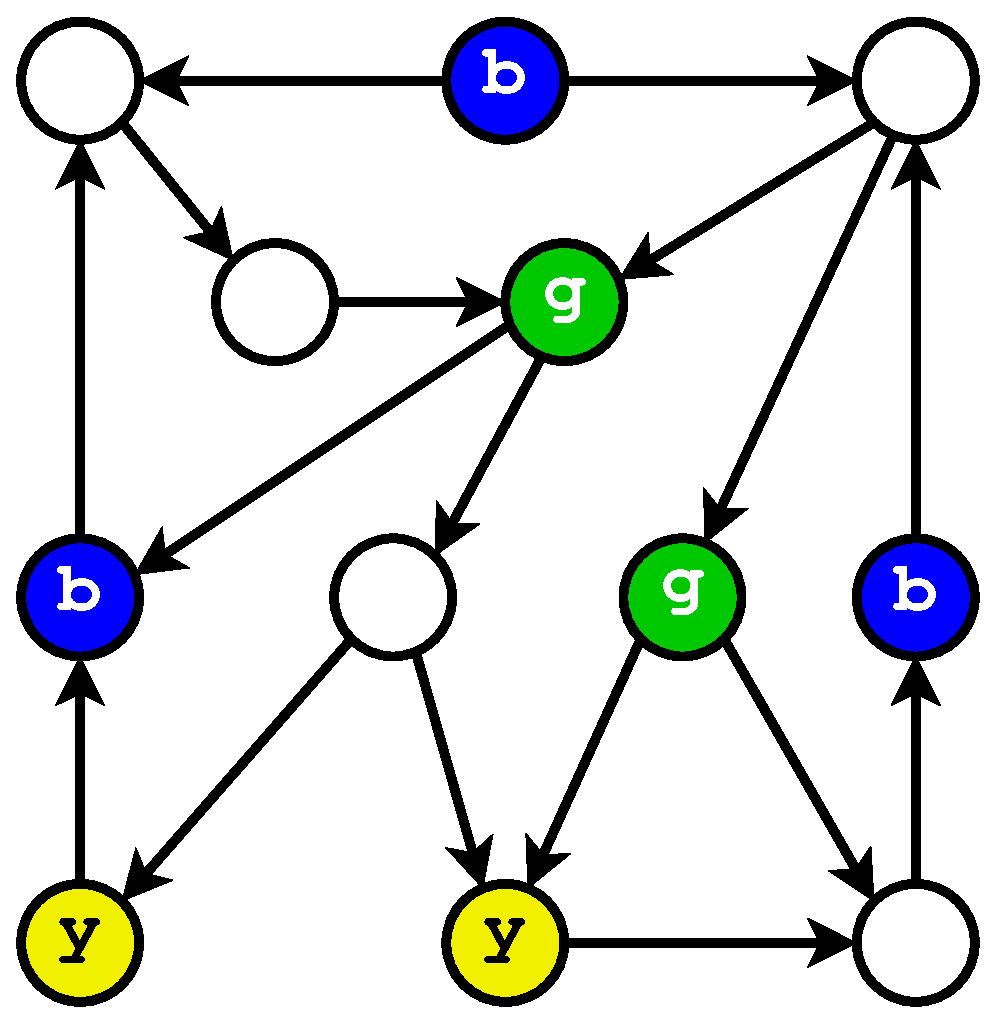
\includegraphics[width=0.75\linewidth]{images/nutshell-answer.eps}
  \caption{Example of an operationally colored graph.}
  \label{fig:imp-ppa}
\end{subfigure}
\hfill
\begin{subfigure}[b]{0.4\textwidth}
  \centering
  \includegraphics[width=0.4\textwidth]{images/nutshell-abstraction.eps}
  \vspace{3ex}
  \caption{Path predicate abstraction graph of Fig.~\ref{fig:imp-ppa}.}
  \label{fig:abs-ppa}
\end{subfigure}
\caption{Example of an Operational coloring of graphs. Implementation automata $M$ in~\ref{fig:imp-ppa} and its corresponding abstraction automata $\hat{M}$ in~\ref{fig:abs-ppa}. (Reprinted from \cite{paper-pdd})}
\label{fig:oper-graph}
\end{figure}

As stated in \cite{paper-pdd}, the coloring of the operational graph has the following attributes:

\begin{itemize}
\item All operational paths are finite. Hence, every cycle in the graph must include at least one colored node. 
\item All nodes of the same color allow for the same set of operation. In other words, if there exists an operational path from node colored $A$ to node colored $B$, then, for any node colored $A$, there is an operational path to some node colored $B$.
\end{itemize}

This “\textit{operational coloring}” allows the abstraction of the implementation graph. Since the colored nodes of the same color support the same operations, they can be abstracted as a single node. In addition, the white nodes are removed, and all corresponding operations collapsed into a single edge. As a result, an abstraction graph can be derived from the implementation graph and they both comprise the same set of operations, i.e. they are equivalent.

The direct graphs may be interpreted as a finite state transition structure such as Kripke Model or an FSM. In \cite{paper-pdd} the Kripe models are translated into FSMs. Then, the Kripke states become a set of three separated coloring functions applied to objects of the RTL implementation:

\begin{enumerate}
    \item A function that maps a subset of the FSM states to states colors $\hat{S}$;
    \item A function that maps input sequences to input colors $\hat{X}$ ; 
    \item A function that maps output sequences to output colors $\hat{Y}$.
\end{enumerate}

These colors serve as elements of an abstract FSM $\hat{M} = (\hat{S}, \hat{s}_{reset}, \hat{X}, \hat{Y}, \hat{\delta}, \hat{\lambda})$. Reading the graph in Fig.~\ref{fig:oper-graph} as an FSM, it means that, for any sequence of input colors, the implementation FSM and the abstract FSM produce the same sequence of output colors. This is called “\textit{sequential equivalence in terms of colors}”.

Even though the abstraction, i.e. the coloring, can be done in different ways, the coloring functions have to follow the operational coloring requirements stated in \cite{paper-ppa}.

Finally, as stated in \cite{paper-pdd}, in practice, the operational coloring is established through formal property checking. Thus, every operation of the design must be described as a property, creating a complete set of operation properties. Any property that can be expressed in terms of colors will be valid for both abstraction and implementation.

\subsubsection*{SystemC-PPA}

\textit{SystemC-PPA} is a subset of \textit{SystemC} \cite{lib-systemc}. According to Ludwig et al. \cite{paper-pdd}, the restriction to a subset is needed because \textit{SystemC} lacks clear semantics with respect to modelling digital hardware. Writing SystemC-PPA compliant modules results in an executable system-level design that also matches the semantic of the formal model of \cite{paper-pdd}. The usage of SystemC-PPA and how it is inserted on the PDD flow is detailed in Sec.~\ref{subsection:PDD-flow}.

The way a SystemC-PPA module is structured allows its behaviour to be extracted as a PPA. In order to achieve that, modules should adhere to the following guidelines:

\begin{enumerate}
    \item model an FSM in a time-abstraction fashion;
    \item have a single thread executing infinitely;
    \item communicate only through an allowed set of communication interfaces;
    \item only block upon a call to a blocking communication interface;
    \item not have cyclic execution path without blocking communication;
    \item use only objects whose size is known at compile time.
\end{enumerate}

As stated in the guidelines, SystemC-PPA modules are allowed to a specific set of communication interfaces, or \textit{ports}. There are three kinds of ports available that aim to provide enough flexibility to model any type of hardware communication at the RTL level. The first one is the \textit{blocking} interface which implements a blocking message passing \textit{handshake}, and it ensures that there is no message loss. The second type is called \textit{Master/Slave} interface. It should be used when the slave side is known to be always ready to communicate. In this case, the master side may communicate without having to synchronize. The last type is named \textit{Shared} interface which does not implement any \textit{handshake} mechanism. Therefore, the \textit{Shared} interface is able to model the behaviour of volatile memory and it fits for modelling unordered input data like sensor values. 

\begin{figure}[htb!]
    \begin{lstlisting}[language=C++]
    struct Example : public sc_module {
        //Constructor
        Example (sc_module_name name):
            value(9) {SC_THREAD (fsm);}
        SC_HAS_PROCESS(Example);
    
        //Ports
        blocking_in<int> b_in;
        blocking_out<bool> b_out;
    
        //Variables
        int value;
    
        //Finite State Machine
        void fsm(){
        while(true){
            b_in->read(value);
            if (value < 10){
                b_out->write(true);
            }else b_out->write(false);
        }}
    };\end{lstlisting}
    \caption{Example of a module written in SystemC compliant to the SystemC-PPA semantics. The module is intended as a toy example and simply reads a integer value through a \textit{blocking} port, and writes \textit{true} to a Boolean output, also of the \textit{blocking} type, if the value is lower than 10 or writes \textit{false} otherwise. }
    \label{fig:sysc-example}
\end{figure}

Fig.~\ref{fig:sysc-example} shows an example of a SystemC-PPA module extracted from \cite{descam}. The module has a single thread that runs infinitely, called\textit{ fsm()}. There are two communicating ports of the \textit{blocking} interface type; an input $b\_in$ and an output $b\_out$. These ports allow the module to communicate through blocking method-calls, for instance, the \textit{read()} and \textit{write()} at lines 17 and 19. 

To conclude, SystemC-PPA does not place any restrictions on which types of hardware behaviour can be modelled, but \textit{how} it should be described.

\subsection{The PDD flow}
\label{subsection:PDD-flow}

The complete flow of the Property-Driven Design methodology proposed in \cite{paper-pdd} is depicted in Fig.~\ref{fig:pdd-flow}. The starting point for the design process is an ESL description of the system. Already in the system-level, first refinements should be made in order to create a system-level model from which the PPA can be extracted, i.e. clear semantics with respect to PPA, or a SystemC-PPA compliant description. This refined description is said to be at the \textit{architectural-level}. 

\begin{figure}[htb!]
	\centering
	\includegraphics[width=0.85\textwidth]{images/design-flow.pdf}
	\caption{Design flow for the PDD methodology. (Reprinted from \cite{paper-pdd})}
	\label{fig:pdd-flow}
\end{figure}

At the architectural-level, the system behaviour is described in terms of data manipulation between communication points. In other words, the important states corresponds to the communication transactions, and an operation describes the data path between communication points. The communication is modelled in a time-abstract way. 

The second step of the design flow starts with the generation of abstract properties. Each property specifies an operation of the design, and for each module of the system, a set of properties is generated. These properties describe the \textit{I/O} behaviour that maps the communication primitives employed in the abstract design to the corresponding communication schemes at the RTL, as detailed in \cite{paper-pdd}. There are three types of properties generated for the property set in this step:

\begin{enumerate}
\item Reset Property: it is a special operation that describe the design behaviour and state after reset.
\item Regular Property: describe the behavior of a regular operation between communication points.
\item Wait Property: generated for each blocking port. Upon the wait for a synchronization signal in a blocking message transfer, this operation guarantees that the design remains at the same state.
\end{enumerate}

For the third step, the design flow splits into two threads. The thread on the left side of Fig.~\ref{fig:pdd-flow} refers do the RTL design process which defines the implementation of a \textit{cycle-accurate} RTL design from an abstract implementation. This corresponds to the conventional RTL design process, and all common design practices can be applied. In addition, any solution regarding the micro architectures of the system can be chosen.

The thread on the right side of Fig.~\ref{fig:pdd-flow} formally describes what is implemented by the left side through a set of properties that constitute a “\textit{formal data sheet}” of the design. This formal description provides the formal proofs that anchor the soundness of the system model and therefore the correctness of the design refinements. The properties are initially generated in terms of macros and functions. During this step of the design process, a \textit{refine-and-implement} cycle is established between the two threads. While the RTL is implemented, the property set must be refined to include the implementation details by updating the generated macros and functions. In order to ensure the correct refinement, the designer must change the properties by filling this set of fields.

During the \textit{refine-and-implement} process, the property suite can be checked against the RTL implementation, and found mismatches can be debugged. The system-level description is a sound path predicate abstraction of the RTL design, guaranteed by formal verification, when at least all the generated properties have been proved correct on the RTL code.

\subsubsection*{DeSCAM}

The authors in \cite{paper-pdd} have implemented a tool to support PDD methodology, called \textit{DeSCAM} (Design from SystemC Abstract Models) \cite{descam}. This tool is primarily essential on the step two of PDD flow for automatically generating the abstract property suit. However, it was designed in order to assist the designer through the entire PDD flow.

Starting with an abstract ESL description of the system, the tool can analyse and give the designer feedback to help refining the initial system-level model into a model at the architectural-level, which is PPA compliant. After having a correct SystemC-PPA description of the system, DeSCAM automatically generates the abstract property set to be refined by the designer. To assist even further, DeSCAM can optionally generate templates in HDL for the main control structures of the system that can be used as a starting point for the RTL implementation.

For each type of communication interface, the tool will generate a specific set of signals for both properties macros and HDL template. A \textit{blocking} interface will generate one signal of the port datatype for transporting the message content, and two more synchronization Boolean signals to implement the four-phase \textit{handshake} behaviour. One outgoing signal to start the handshake tagged with the \textit{notify} suffix, and a incoming signal tagged with the \textit{sync} suffix which informs that the other side is ready to communicate. The \textit{Master/Slave} interface only needs the data signal for the message and one synchronization signal; an outgoing \textit{notify} for the \textit{Master} port and incoming \textit{sync} for the \textit{Slave} port. The \textit{Shared} interface does not require any synchronization signal.

Regardless the of facilitation provided by the tool, the PDD methodology proposed in \cite{paper-pdd} can be applied without any restrictions on the RTL design with respect to architecture, implemented functionality, micro architectural optimizations and coding style. 
